%% Lee
%% In dissertation, change 
%    section* to chapter 
%    subsection* to section
%    subsubsection* to subsection

\chapter{Artificial Neural Networks}
%\section{Artificial Neural Networks}
\label{sec:chap-two}

Recently, there has been much interest in the use of artificial neural networks in systems that employ tasks such as image recognition\cite{krizhevsky2012imagenet}, text recognition\cite{qiu2013parallel} and game playing\cite{maddison2014move}.
In particular, in the field of image recognition these artificial neural network models have demonstrated superior performance
over other state-of-the-art technology\cite{krizhevsky2012imagenet}.
%There is reason to believe 
These artificial neural networks will continue to be applied to numerous other areas such as voice recognition, text recognition, 
face recognition and autonomous control.

Artificial neural networks (\ac{ann}) take their inspiration from neuron behavior observed in the mammalian brain, although implementations are simplifications of what actually exists in the brain.

The mammalian neuron is a cell that receives input and generates output in the form of electrical and chemical processes.
The neuron has a cell body (or soma), a group of dendrites which provide the inputs from other cells, a cell body, an axom which generates the output signals, and the axom terminals which are the outputs of the cell.
The connection from a cells output, or axom terminal to another cells input, or dendrite is known as a synapse. 
The connection in the synapse is a chemical process stimulated by electrical impulses.
The neuron can be seen in figure \ref{fig:neuron}.

The connection from one cell to another has both an associated delay and a strength. The strength of the connection can be influenced by the size of the pre-synaptic neuron spike or by the pre-synaptic neuron generating a series of spikes rather than a single spike.

\begin{figure}[!t]
% the [] contains position info e.g. [!t] means here
\centering
\captionsetup{justification=centering}
\captionsetup{width=.9\linewidth}
\centerline{
\mbox{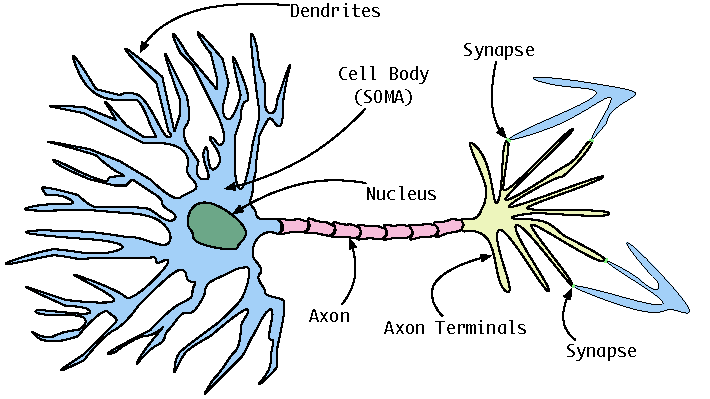
\includegraphics[width=4.0in]{Neuron.pdf}}
}
\caption{Artists impression of a Mammalian Neuron}
\label{fig:neuron}
\end{figure}



\iftrue
So it is known that mammalian neurons generate "spikes" in response to inputs which for humans include sight, touch, sound etc.. This spiking behavior is often referred to as the neuron being activated.
When these neurons are activated, their spikes propagate to other neurons. Under certain conditions, the combination of the various inputs to a neuron cause it to activate. 
A particular neuron may have many hundreds, perhaps thousands of other neurons connected to its "input".
These input neurons are referred to as pre-synaptic neurons. These pre-synaptic neurons may provide input to many neurons which are referred to as post-synaptic neurons.
A particular neuron can get activated by a particular arrival pattern of pre-synaptic neuron spikes or simply by the intensity of the pre-synaptic spikes. 

The spiking behavior of a neuron also varies and many spiking profiles have been observed, including single spikes, groups of spikes and repetitive spiking. 
It is believed that information is carried in the delay and strength of the connections and how pre-synaptic neurons combine to cause a neuron to activate.
In simple terms, if a neuron is activated by its pre-synaptic neurons, then the activation of the neuron means a pattern has been detected which will influence a reaction.
In mammalian terms, that might be the detection of a threat from both smell and sight neurons and the reaction is to control muscles resulting in flight.


The various chemical and electrical processes that result in the generation and propagation of these neuron spikes is beyond the scope of this dissertation, but how neurons and networks of neurons are artificially emulated is what we will discuss next.


%\section[NnSP]{NnSP{\cite{esmaeilzadeh2005nnsp}}}
\section[Artificial Neural Networks]{Artificial Neural Networks}
\label{sec:Artificial Neural Networks}

When modeling these neurons in artificial neural networks, the neuron models either generate actual spikes similar to actual neurons or
produce a value which is proportional to the rate at which spikes occur.
These artificial neural networks can be categorized as rate-based coded or spike time coded neurons.


When used in networks of neurons, both model types employ a connection weight between the pre and post-synaptic neuron, however, the spiking neuron network also introduces a time delay associated with the connection.

The spiking neuron model is characterized by:

\begin{outline}
  %\setlength{\baselineskip}{10pt}
  %\setlength{\itemsep}{12pt}
  %\setlength{\partopsep}{0pt}
  %\setlength{\parskip}{0pt}
  %\setlength{\parsep}{0pt}
  %\setlength{\topsep}{0pt}
  %\setlength{\itemindent}{\leftmargin}
  %\setlength{\leftmargin}{0pt}
        \1 Connections between neurons have both a strength and a delay
          \2 The pre-synaptic neuron output is multiplied by the connection weight and delayed
        \1 The weighted inputs from all pre-synaptic neurons are accumulated
        \1 The accumulated inputs drives an activation function
          \2 the activation function $f(x)$ is a spiking model is based on differential equations
          \2 many models have been proposed with varying levels of complexity
            \3 examples are:
              \4 Leaky integrate and fire
              \4 Izhikevich \cite{Iz2005} (see \fref{fig:Izhikevich Model})
         
\end{outline}

The Rate-based neuron model is characterized by:
\begin{outline}
        \1 Connections between neurons have only a strength
          \2 The pre-synaptic neuron output is multiplied by the connection weight
        \1 The weighted inputs from all pre-synaptic neurons are accumulated
        \1 The accumulated inputs drives an activation function
          \2 the activation function $f(x)$ is a non-linear function
          \2 early models used binary functions although in practice the function needs to be differentiable
            \3 examples are (see \fref{fig:Example Rated-Based Model Activation functions}):
              \4 sigmoid
              \4 rectified linear unit
\end{outline}

\begin{figure}
\centering
\begin{subfigure}{.4\textwidth}
  \centering
  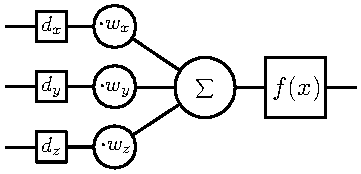
\includegraphics[width=0.85\textwidth]{SpikeBasedModel}
  \captionsetup{justification=centering, skip=5pt}
  \caption[Spiking Model]{Spiking Model}
  \label{fig:simpleNetwork}
\end{subfigure}%
\begin{subfigure}{.4\textwidth}
  \centering
  \includegraphics[width=0.7\textwidth]{RatebasedModel}
  \captionsetup{justification=centering, skip=5pt}
  \caption{Rate-Based Model}
  \label{fig:cellContents}
\end{subfigure}
\begin{subfigure}{.9\textwidth}
  \centering
  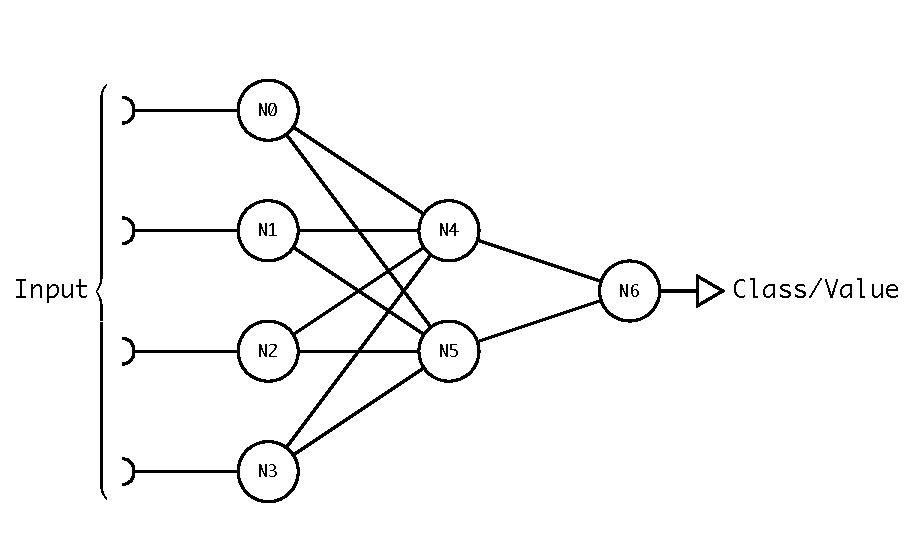
\includegraphics[width=0.7\textwidth]{SimpleNetwork}
  \captionsetup{justification=centering, skip=5pt}
  \caption{Network of Artificial Neurons}
  \label{fig:cellContents}
\end{subfigure}
\captionsetup{justification=centering, skip=6pt}
\caption[Artificial Neural Network]{Artificial Neurons and Network}
\label{fig:Artificial Neural Network}
\end{figure}

\begin{figure}
\centering
\begin{subfigure}{.3\textwidth}
  \begin{tikzpicture}[scale=0.5]
    \begin{axis}[
        title={Sigmoid},
        %grid = major,
        xmin=-6,xmax=6,
        ymin=0,ymax=1,
        legend style={draw=none, fill=white},      
        legend pos= outer north east
        ]
        \addplot[myBlueThickStyle] expression[domain=-6:6,samples=100]{1/(1+e^(-x))} 
                    node at (axis cs:3,0.7){}; 
        \legend{{\large $f(x)=\frac{1}{1+e^{-t}}$}}
    \end{axis}
  \end{tikzpicture}
  \captionsetup{justification=centering, skip=5pt}
  \caption{Sigmoid}
  \label{fig:Sigmoid}
\end{subfigure}%
\begin{subfigure}{.3\textwidth}
  \begin{tikzpicture}[scale=0.5]
    \begin{axis}[
        title={ReLu},
        xmin=-1,xmax=1,
        ymin=0,ymax=1,
        legend style={draw=none, fill=white},      
        legend pos= outer north east
        ]
        \addplot[myBlueThickStyle] expression[domain=0:1,samples=100]{x} node at (axis cs:0.6,0.15){}; 
         \addplot[myBlueThickStyle] expression[domain=-1:0,samples=100]{0};       
         % had to change , to f&%$$#$g \text{,} on max.ece.ncsu.edu, what BS
         \legend  {{ $f(x)= \begin{cases} 0\text{,}      &\text{if $x < 0$;}\\   x\text{,}       &\text{otherwise.}  \end{cases}$}}  
    \end{axis}
  \end{tikzpicture}
  \captionsetup{justification=centering, skip=5pt}
  \caption{Relu}
  \label{fig:Relu}
\end{subfigure}
\captionsetup{justification=centering, skip=5pt}
\caption{Example Rated-Based Model Activation functions}
\label{fig:Example Rated-Based Model Activation functions}
\end{figure}

\begin{figure}
\centering
\captionsetup{justification=centering}
\vspace{0.5cm}
\begin{subfigure}{.9\textwidth}
  \centering
  \begin{equation}
    \begin{split}
    &v' = 0.04v^2+5v + 140 - u - I\\
    &u' = a(bv-u)  \\
    &\text{if } v\ge  \SI{30}{\mV}, \text{ then } 
    \begin{cases}
        v \leftarrow c\\           
        u \leftarrow u+d\\           
    \end{cases} \nonumber
    \end{split}
  \end{equation}
  \caption{Izhikevich Model\cite{Iz2005}}
  \label{fig:Izhikevich Model}
  \end{subfigure}
\begin{subfigure}{.7\textwidth}
  \centering
  \mbox{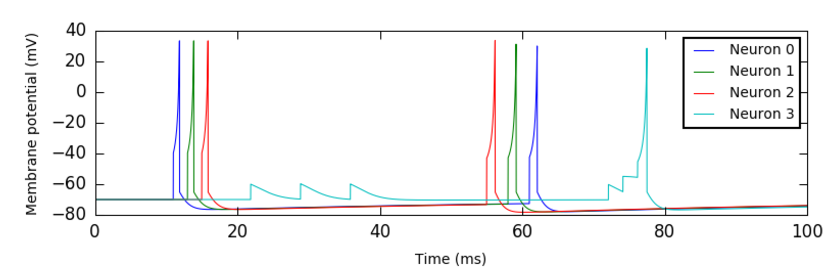
\includegraphics[width=4.0in]{SpikingExample.pdf}}
  \captionsetup{justification=centering, skip=3pt}
  \caption{Izhikevich Model Simulation \cite{Iz2005}\cite{carnevale2006neuron}}
  \label{fig:spiking example}
\end{subfigure}
\caption{Example Spiking Activation Function Model}
\label{fig:Example Spiking Model}
\end{figure}

To emulate complex behavior, the artifical neurons are connected in networks, typically with layers of sub-networks which are in affect separated by the non-linear activation function.
Examples of both rate-based and spiking artificial neural networks can be seen in \fref{fig:Rate-based Model Network} and \fref{fig:Spiking Model Network} respectively.
Typically neural networks process in a feed-forward fashion. Considering \fref{fig:Artificial Neural Network}, this means the input arrives on the left, the inputs propagate to neurons N0 through N3. WHen N0 through N3 are processed, their values propagate forward to neurons N4 and N5 etc.. SOmetime \ac{ann}s also include recursion where for example neurons N0 through N4 are not only influenced
by the input, but also by themselves. Many \ac{ann}s operate only in feed-forward fashion but some popular \ac{ann}s, such as Long short-term memory (LSTM), employ recursion.

Another popular \ac{ann} known as Deep Neural Networks (\ac{dnn}) have proved very popular over the last few years. They get good press in applications such as image recognition and speech recognition. 
Deep Neural Networks are often formed from tens of layers of \ac{an}s with each layer containing many \ac{an}s. \ac{dnn}s are also processed in a feed-forward manner with one layer being the inputs to the next layer. 
As mentioned \cite{krizhevsky2012imagenet}, these useful \ac{dnn}s often require hundreds of thousands of \ac{an}s and within the network, each \ac{an} can have hundreds, even thousands of feeder or pre-synaptic \ac{an}s.
There have been implementations that use different number formats from double precision floating point to eight bit integers, but in all cases these useful \ac{ann}s require a significant amount of memory to store the connection weights (parameters).


\begin{figure}[!t]
  % the [] contains position info e.g. [!t] means here
  \centering
  \captionsetup{justification=centering}
  \captionsetup{width=.9\linewidth}
  \begin{subfigure}{.9\textwidth}
    \centerline{
    \mbox{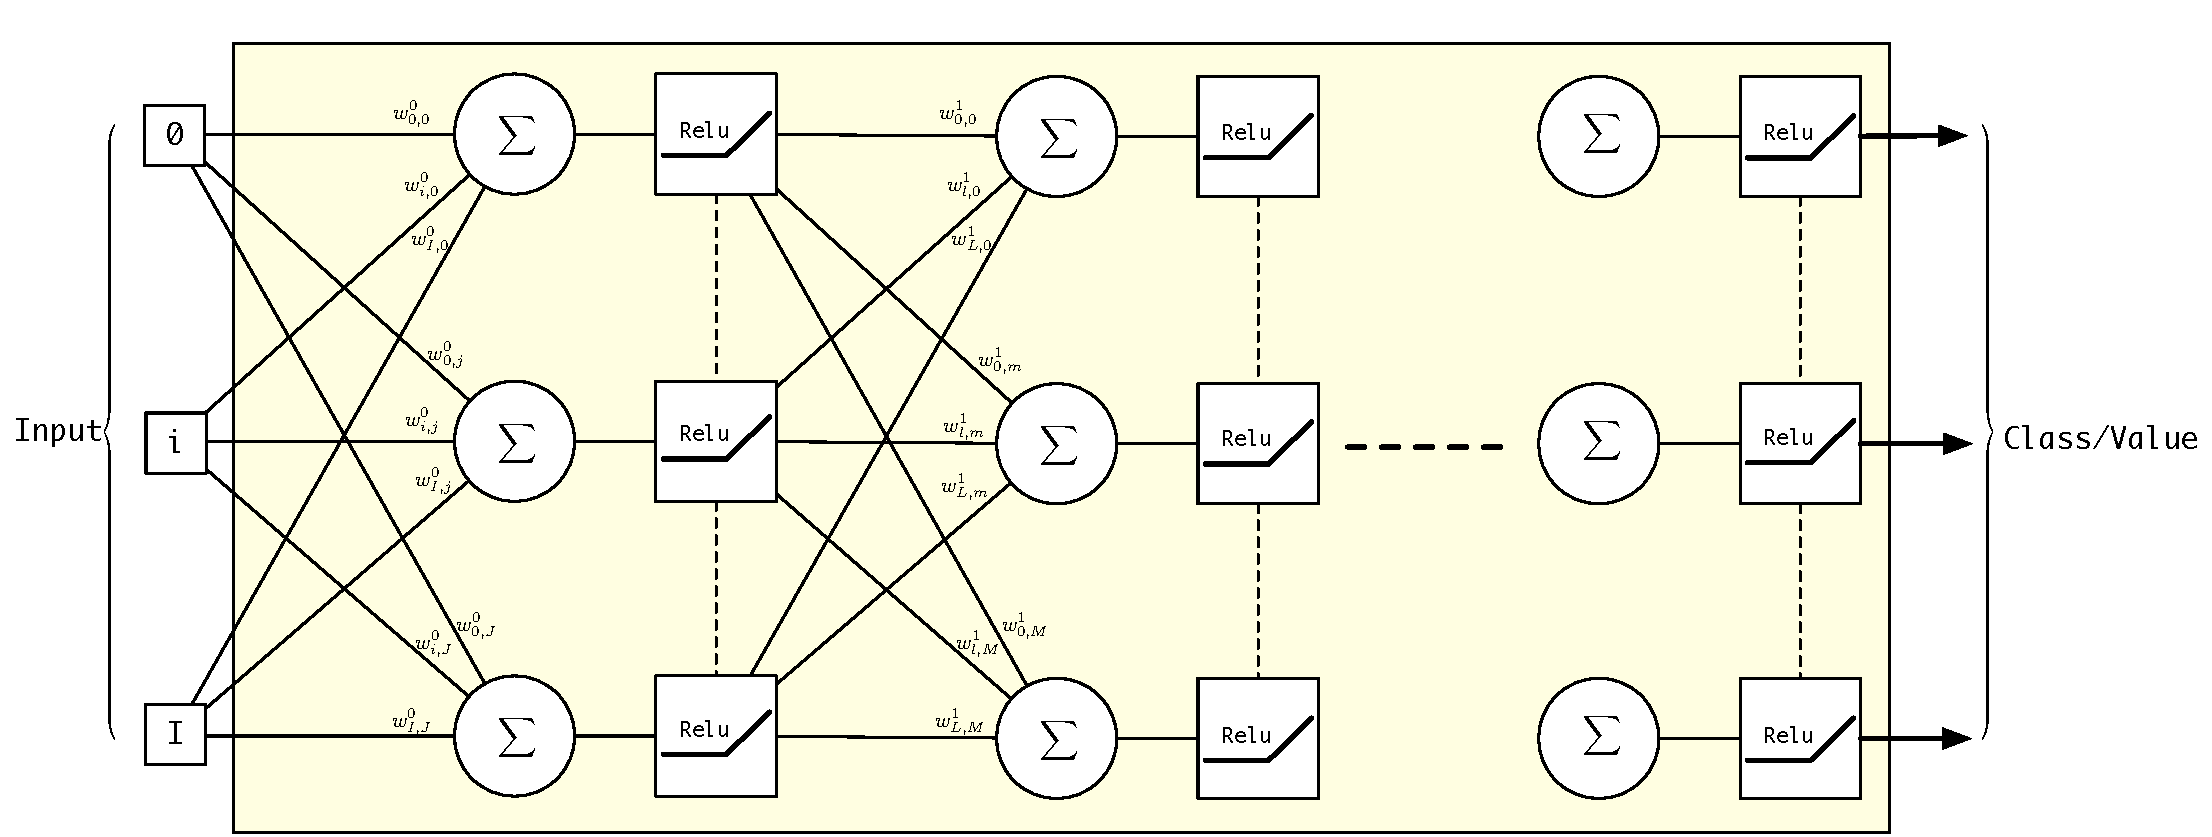
\includegraphics[width=6.0in]{RateBasedNeuralNetwork.pdf}}
    }
    \caption{Rate-based Model Artificial Neural Network (with ReLu activation function)}
    \label{fig:Rate-based Model Network}
  \end{subfigure}
  
  \begin{subfigure}{.9\textwidth}
    \centerline{
    \mbox{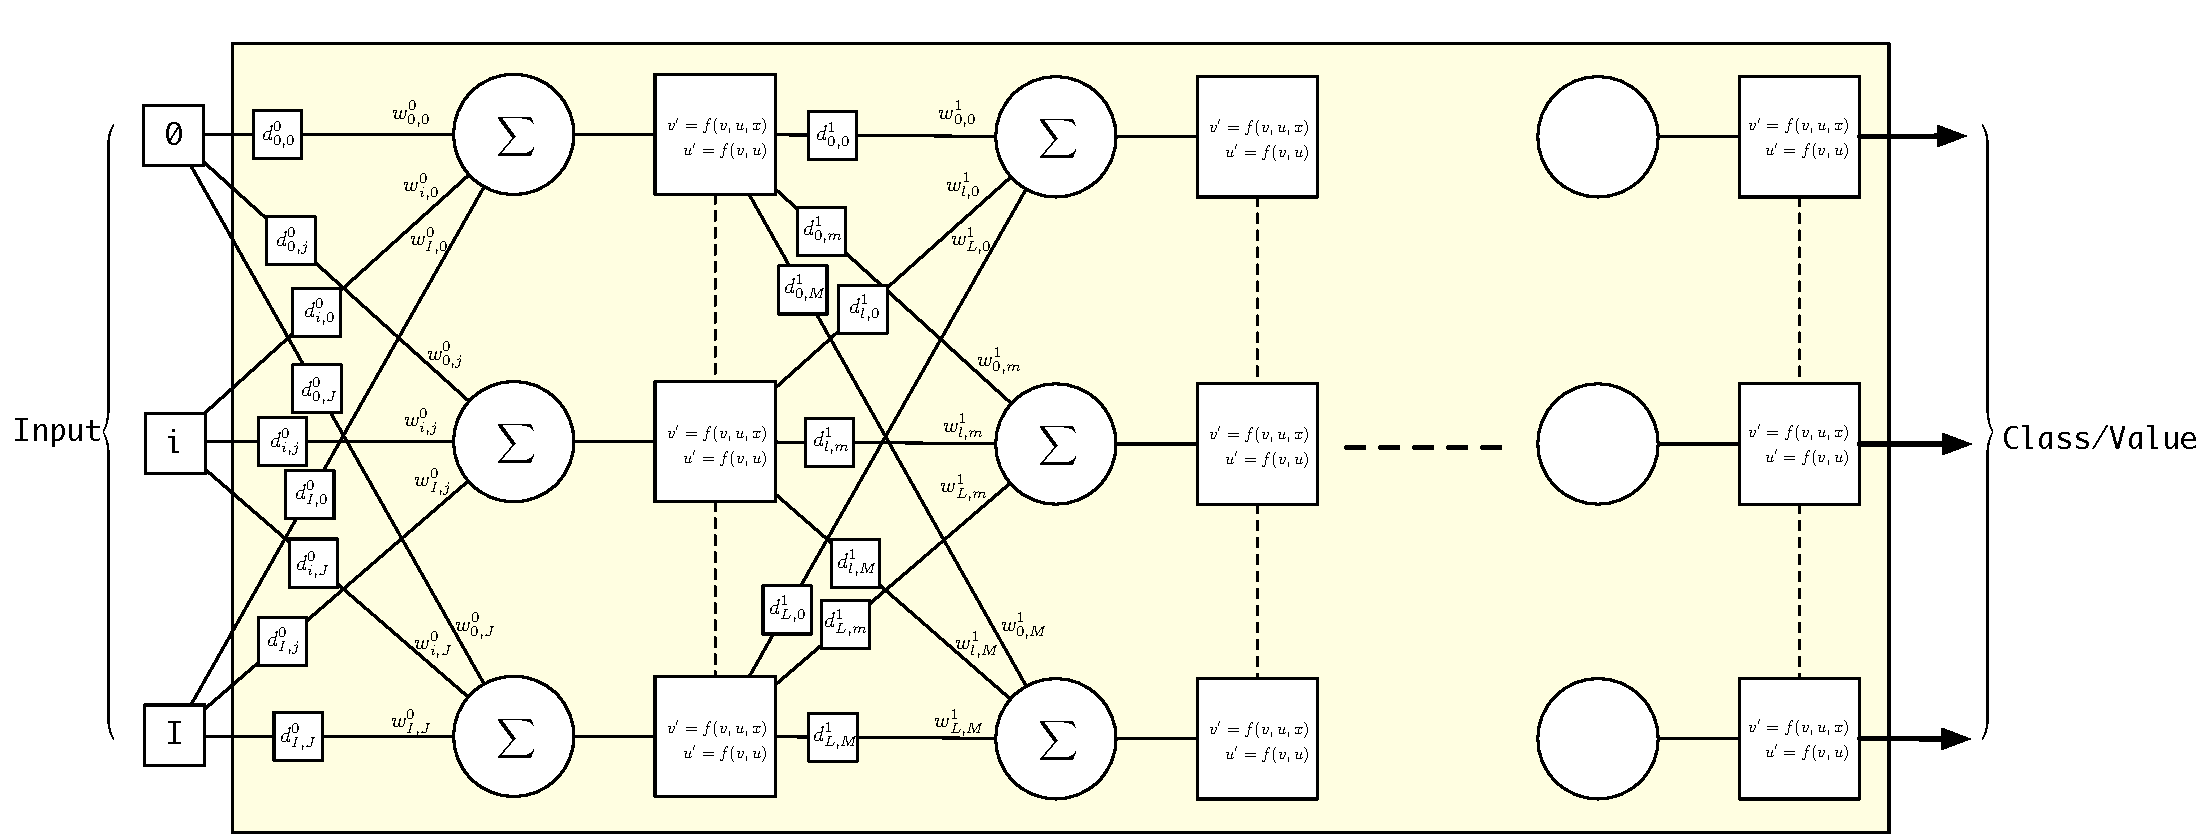
\includegraphics[width=6.0in]{SpikingNeuralNetwork.pdf}}
    }
    \caption{Spiking-based Model Artificial Neural Network}
    \label{fig:Spiking Model Network}
  \end{subfigure}
  \caption{Layered Artificial Neural Networks}
  \label{Example Artificial Neural Networks}
\end{figure}

Although the spiking neural network more closely models the behavior of real neurons, over the last 20 years there 
have been breakthroughs in the configuring of rate-based models especially with the introduction of the back-propagation
algorithm and stochastic gradient descent. Along with the abundance of data now available in the form of voice, images etc. to "teach" these networks
using back-propagation, most of the effective applications of artificial neural networks have employed these rate-based models.

\iffalse
Our research will focus on these rate-based models which we will now refer to as \ac{ann}s.
\fi


\section[The Problem]{The Problem}
\label{sec:The Problem}

To approach the capabilities observed in human behavior, such as object recognition these \ac{ann}s become very large.
They often utilize hundreds of thousands of neurons to implement what a human would consider a relatively straightforward task.
For example, a "useful" \ac{ann} similar to that described in \cite{krizhevsky2012imagenet} that is used to recognize up to 1000 different object classes has a network size of approximately 650,000 neurons and 630 million synaptic connections \cite{krizhevsky2012imagenetPreso}. 

The increased performance of \ac{ann}s over classical methods in image recognition and voice recognition might suggest that \ac{ann}s might out-perform other existing systems in other applications.
There is reason to believe that these \ac{ann}s will replace existing control and monitoring functions in existing systems.

If \ac{ann}s fulfill their potential, systems employing \ac{ann}s will utilize them for various functions, such as engine monitoring, anomaly detection, navigation etc. all within the same system.
Considering the various functions a complex customer facing or edge application system performs, it is likely that many real-world applications will employ multiple disparate instances of these useful sized \ac{ann}s.
Assuming these complex functions will require \ac{ann}s similar in size to \cite{krizhevsky2012imagenet}, these implementations will be processing multiple large \ac{ann}s at or near real-time.

Considering the storage required for the input, the \ac{an} states and most significantly the weights for each of the \ac{an}s, the storage requirements results in gigabytes of memory.
When these \ac{ann}s are required to be solved in fractions of a second, the processing and memory bandwidth becomes prohibitive.

As a metric, this work asumes that any useful \ac{dnn} will employ 100's of thousands of \ac{an}s. Although there is a lot of debate regarding number formats for \ac{ann}s, this work also assumes single-precision floating point.
Assuming an \ac{ann} with 250K neurons and an average fanin to each \ac{an} of 2000, a system employing 10 \ac{ann}s for various disparate functions and an average processing time of \SI{10}{\milli\second} suggests a average bandwidth of \SI[per-mode=symbol]{16}{\tera \bit \per \second} (see equation \ref{eq:averageBandwidth}).

% {2} means 2 columns
\begin{alignat}{2} \label{eq:averageBandwidth}
\text{Average }\text{Bandwidth} & = \sum_{\mathbf{n}=0}^{\bar{\mathbf{N_n}}}\big(\frac{\Bar{\mathbf{N_a}}\cdot \Bar{\mathbf{C_p}} \cdot \bar{\mathbf{b_w}}}{\bar{\mathbf{T_p}}} \big) \notag  \\
& = \sum_{\mathbf{n}=0}^{9}\big(\frac{\num{250d4} \cdot \num{2d3} \cdot 32}{\num{10d-3}} \big) \notag \\
& = \SI[per-mode=symbol]{16}{\tera\bit\per\second} \\
\text{where } &\mathbf{N}_n \text{ is the number of \ac{ann}s} \notag\\
              &\mathbf{N}_a \text{ is the average number of \ac{an}s} \notag\\
              &\mathbf{C_p} \text{ is the average number of connections} \notag\\
\text{and }   &\mathbf{T_p} \text{ is the processing time} \notag
\end{alignat}

Therefore, when imlementing \ac{ann}s, the memory requirements are significant. The storage is required for the input, the \ac{an} state and most significantly the weights for each of the \ac{an}s. This storage requirement often results in gigabytes of memory.

In addtion, in edge applications, it is anticipated that these \ac{ann}s are required to be solved in fractions of a second, in which case the processing and memory bandwidth becomes prohibitive.

The problem becomes \hyphenquote{american}{\textbf{\textcolor{black}{to provide deterministic at or near real-time performance within tolerable power and space constraints for edge systems employing inference on multiple disparate useful-sized neural networks.}}}
%\hlc[gray]{hello}

Considering that DRAM is required to store the NN parameters, why use SRAM as an intermediate store? Well, in practice there are benefits if you can operate solely out of SRAM.
Certainly good performance and potentially low power.
But use of SRAM makes assumptions on the NNs that can be supported and the application.
The primary requirement of the NN to allow effective use of SRAM is "reuse". Once parameters are stored in SRAM, can they be reused such that the SRAM isn't simply an intermediate memory but something akin to a cache.

In some \ac{ann}s there are reuse opportunities. Specifially, with \ac{cnn}s, the weights are reused. A convolutional filter is passed across an input to form the next layer. These filter "kernels" can be held in memory and the input is read from DRAM thus reducing the DRAM bandwidth.
Even with \ac{dnn}s where weights may not be reused, when implementing multiple \ac{dnn}s, there is opportunity to hold the input in memory.
If the system is being employed in cloud applications or in training, there is opportunity to reuse inputs whilst performing batch processing.

But SRAM comes at a price, its big. Often when we see physical layouts of NN processors, they are dominated by the silicon area of the SRAM. The area required for SRAM has been understood for quite some time and companies attempt to create custom SRAMs to minimize the area impact.

So the question becomes, can a system employ DRAM with minimal SRAM and still provide a high performance system within acceptable area constraints?

\iffalse
We believe a system can be designed with DRAM as the primary processing store. This will require careful use of data structures to describe storage within DRAM to ensure we make good use of the potential bandwidth. But there are other benefits we will take advantage of, but more about that later.
\fi

\iffalse
There important application is disparate \ac{ann}s because specifically a form of \ac{dnn}, Convolutional Neural networks (\ac{cnn}) have gotten good press recently, but they are not the only \ac{dnn}.
\fi

Even in cloud applications, there are limitations on reuse. We paraphrase a quote from a Google paper \cite{tensorflow2015-whitepaper} on their Tensor Processing Unit ASIC (TPU):

\hyphenquote{american}{the architecture research community is paying attention to NNs, but of all the papers at ISCA 2016 on hardware accelerators for NNs, alas, all nine papers looked at \ac{cnn}s, and only two mentioned other NNs. Unfortunately \ac{cnn}s represent only about 5\% of our datacenter NN workload}

The applications targeted by the google TPU \cite{tensorflow2015-whitepaper} assume multiple requests, so reuse in the form of batch processing is still of great benefit, but the bulk of the requests in \cite{tensorflow2015-whitepaper} are fully-connected \ac{dnn}s and in these cases weight reuse is not as benefitial and the performance of the TPU is degraded when implementing these fully-connected \ac{dnn}s.

Therefore, implementations that focus on \ac{cnn}s can suffer from severe degradation in performance when targeting generic types of \ac{ann}, such as locally and fully connected \ac{dnn}s and LSTMs.

This work focuses on edge applications employing disparate \ac{ann}s and assumes both weight reuse and batch processing do not apply.
Considering systems will want to perform multiple \ac{dnn}s simultaneously suggests that these edge systems will require usable memory bandwidth of the order of 10's of \SI[per-mode=symbol]{}{\tera \bit \per \second}.

In these cases, \textbf{\textcolor{black}{DRAM bandwidth is the bottleneck}}.




\iffalse
So considering the performance improvements observed in other applications, it is expected that many customer facing or edge applications will implement multiple instances of artificial neural networks to perform various functions.
have very large memory and processing requirements.
require multiple instances of \ac{ann}s of similar size to the \ac{ann} described in \cite{krizhevsky2012imagenet}.

For example employing multiple cameras or monitoring and controlling different systems in a drone, a automobile each with an image recognition \ac{ann}\cite{krizhevsky2012imagenet}\cite{bojarski2016end} for navigation, engine monitoring along with other system control.
\fi

Some might suggest the requirements of these applications would be satisified by employing multiple graphics processor units(GPU).
In fact, Graphics processing Units (GPU) are used to implement large \ac{ann}s and in some \ac{ann} architectures, such as Convolutional NNs (\ac{cnn}), they are quite effective. However, we should not forget they are not optimized purely for \ac{ann} processing and are restricted by available SRAM and they are power hungry. These limitations will limit the effectiveness of GPUs regardless of what we might hear from the GPU community.
Even in the case of newer GPUs which are employing 2.5DIC technology, the memory bandwidth will still be limited by available DRAM tecnology.
For example, a 2.5D solution employing High bandwidth Memory (HBM) would be limited to a maximum raw bandwith of the order of \SI[per-mode=symbol]{4}{\tera \bit \per \second}.
Also, its has proven very difficult, if not impossible to take advantage of the available memory bandwidth \cite{farabet2011neuflow} \cite{tensorflow2015-whitepaper}.
Given these multiple GPU systems have high real-estate and power requirements and given each instance consumes of the order of \SI{100}{\watt} to \SI{200}{\watt}.
Overall GPUs have limited suitability to meet edge application requirements.


Much of the \ac{ann} application specific (ASIC/ASIP) research has focused on taking advantage of the performance and ease of use of Static Random Access Memory or SRAM. These implementations can be shown to be effective with specific \ac{ann} architectures (\ac{cnn}), server applications or the "toy examples" but when a system requires multiple disparate \ac{ann}s in an edge application, these implementations do not provide the required flexibility, storage capacity and deterministic performance.


\section[The Solution]{The Solution}
\label{sec:The Solution}

Most researchers acknowledge that realistically, DRAM is required to meet the main storage requirements of useful sized \ac{ann}s.

We further believe that to support all types of disparate \ac{ann}s, we need to be able to operate directly from the DRAM memory.

This is because SRAM-based solutions assume memory locality when processing a neural network. However, when \ac{ann}s do not provide sufficient locality these solutions become DRAM bandwidth bound. If we then ensure the DRAM can feed the SRAM at the necessary bandwidth, why use an SRAM and waste the significant silicon area they require.

This works system operates directly from DRAM, but not just DRAM, 3D-DRAM.

In addition, this work has designed a system that can stay within the physical footprint of the 3D-DRAM.

By ensuring the system stays physically within the 3D stack, we take advantage of high density connectivity provided by TSVs. 
Therefore, this work is able to propose a custom 3D-DRAM that exposes more of the DRAMs internal page and thus generates interface bandwidth that is of the order of 64 times that of the standard 3D-DRAM.

\subsection[Novelty]{Novelty}
\label{sec:Novelty}

The novelty of this work includes:
\begin{outline}
    \1 A custom 3D-DRAM providing a ~64X bandwidth benefit compared to standard 3D-DRAM
    \1 A system that benefits from the power and performance benefits of 3DIC technology by remaining within a 3DIC stack
    \1 New data structures that allow use to operate directly out of DRAM whilst ensuring effective use of DRAM bandwidth
    \1 A system that can simultaneously process multiple disparate \ac{ann}s at or near real-time
\end{outline}


This research explores a 3DIC solution using a custom organized 3DIC memory in conjunction with unique data structures and custom processing modules to significantly reduce the 
area and power footprint of an application that needs to support the processing associated with multiple \ac{ann}s.
This works system will provide at or near real-time performance required for systems employing multiple disparate \ac{ann}s whilst staying within acceptable area and power limits and will provide greater than an order of magnitude benefit over comparable solutions.

%%---------------------------------------------------------------------------------------------------------
%%---------------------------------------------------------------------------------------------------------


